\chapter{Experimentos y resultados}
\label{cap:experimentos}

En este capítulo evaluamos el clasificador contextual. Primero describimos la configuración experimental y recordamos las métricas que usamos. Después mostramos los resultados sobre el conjunto principal de estudio, los analizamos familia por familia, los comparamos con una línea base de aprendizaje automático (Machine Learning) y comprobamos su comportamiento en otras semanas del dataset. El capítulo termina con una discusión y unas conclusiones.

Todas las cifras provienen de los ficheros de resultados del proyecto.

\section{Configuración experimental}
\label{sec:exp_configuracion}

La evaluación se realiza sobre el dataset UGR'16 \cite{ugr16}, con tráfico NetFlow real etiquetado. El \textbf{conjunto principal de estudio} es \texttt{august.week1}, la semana sobre la que se formularon las reglas. Las pruebas de \textbf{generalización} se hacen sobre \texttt{august.week2} y \texttt{april.week2}, que no se usaron para diseñar las reglas. En todos los casos, las \textbf{etiquetas del dataset se usan solo para evaluar}.

La elección de cada semana responde a qué ataques contiene. Se tomó \texttt{august.week1} como semana de diseño porque es la que reúne, con un número de trazas suficiente, casi todas las familias del núcleo (escaneo UDP, escaneo vertical \texttt{scan11} y \texttt{scan44}, \texttt{dos} y \texttt{nerisbotnet}), lo que permite estudiar su comportamiento y formular las reglas sobre un mismo conjunto. Las otras dos semanas se reservan para comprobar si esas reglas se sostienen sobre tráfico que no se usó en el diseño. \texttt{august.week2} aporta otra muestra del núcleo de escaneos en un periodo distinto, y \texttt{april.week2} se eligió específicamente porque concentra el escaneo SSH, casi ausente en agosto, y es la única forma de evaluar de manera representativa el tercer pase de la v5.

El clasificador principal es la versión \textbf{v5}. La versión \textbf{v3} se conserva como base estable y sirve de referencia, y la \textbf{v4} fue una prueba que no se adoptó como solución final. La evaluación se hace a nivel de flujo (cada traza recibe una decisión) y los resultados se vuelcan en ficheros de resumen por versión y por semana. La Tabla~\ref{tab:exp_config} recoge los conjuntos de evaluación y sus tamaños.

\begin{table}[ht]
\centering
\small
\begin{tabular}{|l|r|p{6.0cm}|}
\hline
\textbf{Conjunto} & \textbf{Trazas evaluadas} & \textbf{Papel} \\
\hline
\texttt{august.week1} & 6\,870\,331 & Conjunto principal de estudio: formulación de reglas y evaluación principal. \\
\hline
\texttt{august.week2} & 768\,000 & Generalización: familias del núcleo en otra semana. \\
\hline
\texttt{april.week2} & 400\,000 & Generalización: contiene sobre todo escaneo SSH. \\
\hline
\end{tabular}
\caption{Conjuntos de evaluación a nivel de flujo y su tamaño en número de trazas. El conjunto principal se usa para formular y evaluar las reglas. Los otros dos se reservan para la generalización.}
\label{tab:exp_config}
\end{table}

La entrada de la evaluación son las ventanas extraídas de UGR'16 (Capítulo~\ref{cap:algoritmos}). La salida se organiza en cuatro tipos de artefacto. El primero es un \textbf{resumen binario}, con los recuentos de confusión (VP, FP, FN y VN) y las métricas de ataque frente a tráfico normal. El segundo es un \textbf{resumen por familia y subtipo}, con las trazas predichas, las etiquetadas y los aciertos de cada clase. El tercero recoge los \textbf{resultados de generalización}, con esa misma estructura sobre otras semanas. El cuarto es la \textbf{comparación con los modelos clásicos} de aprendizaje automático. El detalle por traza, una fila por flujo con su decisión, familia, subtipo, confianza y señal, se conserva aparte para poder inspeccionar casos concretos. Todos estos artefactos forman parte del material complementario.


\section{Métricas de evaluación}
\label{sec:exp_metricas}

Las métricas se definieron en el Capítulo~\ref{cap:conceptos}. Aquí solo recordamos cómo se aplican. Para la decisión \textbf{binaria} (ataque frente a tráfico normal) se calculan precisión y recall a partir de los verdaderos positivos (VP), falsos positivos (FP) y falsos negativos (FN), y se resume con la medida $F_1$ \cite{sokolova2009systematic}. Un \textbf{falso positivo} es tráfico normal marcado como ataque (una falsa alarma) y un \textbf{falso negativo} es un ataque que se escapa.

La evaluación se hace en dos niveles. El nivel \textbf{binario} mide si el sistema separa bien el ataque del tráfico normal. El nivel \textbf{por familia} mide, para cada tipo de ataque, qué parte de lo predicho es correcta (precisión) y qué parte de lo etiquetado se recupera (recall). Las cifras por familia se obtienen de los recuentos del resumen (trazas predichas, trazas etiquetadas y aciertos) de cada clase.

La \textbf{exactitud} (\emph{accuracy}) no se usa como métrica principal por el fuerte desbalanceo. En el conjunto principal de estudio, de 6\,870\,331 trazas evaluadas, solo un pequeño porcentaje son ataques, así que un sistema que marcase todo como normal obtendría una exactitud altísima sin detectar nada. Por eso se da prioridad a precisión, recall y $F_1$, que reflejan mejor la detección sobre las clases minoritarias.

\section{Evaluación del clasificador contextual}
\label{sec:exp_v5}

La Tabla~\ref{tab:exp_binaria} muestra la detección binaria sobre \texttt{august.week1}, el conjunto principal de estudio, para la base estable v3 y para la versión final v5.

\begin{table}[ht]
\centering
\small
\begin{tabular}{|l|c|c|c|l|}
\hline
\textbf{Versión} & \textbf{Precisión} & \textbf{Recall} & \textbf{F1} & \textbf{VP/FP/FN/VN} \\
\hline
v3 (base estable) & 0,930 & 0,991 & 0,960$^{*}$ & 1\,816\,688 / 137\,365 / 17\,228 / 4\,899\,050 \\
\hline
v5 (final) & 0,926 & 0,991 & 0,957 & 1\,816\,688 / 145\,702 / 17\,228 / 4\,890\,713 \\
\hline
\end{tabular}
\caption{Detección binaria (ataque/normal) en \texttt{august.week1} para la base estable v3 y la versión final v5. $^{*}$El resumen de la v3 no almacena el F1, que se obtiene de su precisión y recall.}
\label{tab:exp_binaria}
\end{table}

En la última columna, los \textbf{VP} son ataques correctamente detectados, los \textbf{FP} tráfico etiquetado como normal que el clasificador marca como ataque, los \textbf{FN} ataques que el clasificador no detecta y los \textbf{VN} tráfico normal clasificado correctamente.

Las dos versiones separan bien el tráfico de ataque del tráfico normal, con un recall de 0,991 en los dos casos. Aun así, hay un matiz: en el conjunto principal de estudio, la v5 obtiene una precisión ligeramente \emph{menor} que la v3 (0,926 frente a 0,930). La causa está documentada en el propio resumen: el tercer pase de detección SSH de la v5 genera 8\,389 predicciones adicionales que, en esta semana, se contabilizan como falsos positivos añadidos por ese pase, porque \texttt{august.week1} apenas contiene escaneo SSH etiquetado. Ese tercer pase agrega por origen el tráfico hacia el puerto 22 (el fan-out de cada origen) y puede reclasificar como escaneo flujos que el contexto local no había marcado. Es lo que permite recuperar el escaneo SSH en \texttt{april.week2}, pero a cambio añade falsas alarmas cuando ese mismo patrón de fan-out aparece en tráfico etiquetado como \emph{background}. Por eso el pase tiene un coste en precisión en las semanas donde ese ataque no está etiquetado, un coste que se compensa en \texttt{april.week2}, como se verá en la sección de generalización.

Además, un falso positivo no siempre es tráfico completamente normal. En esta evaluación se respeta la etiqueta original del dataset: si una traza aparece como \emph{background} y el clasificador la marca como ataque, se cuenta como falso positivo. Sin embargo, en tráfico real puede haber comportamientos anómalos que no hayan sido etiquetados originalmente como ataque. Por eso, algunas de estas alertas podrían corresponder a flujos con una estructura parecida a la de un ataque, aunque el sistema que generó las etiquetas del dataset los dejase dentro del tráfico de fondo. En este trabajo no se corrigen esas etiquetas ni se usan para mejorar artificialmente las métricas, pero sí se consideran una posible explicación de parte de las falsas alarmas.

\begin{figure}[ht]
\centering
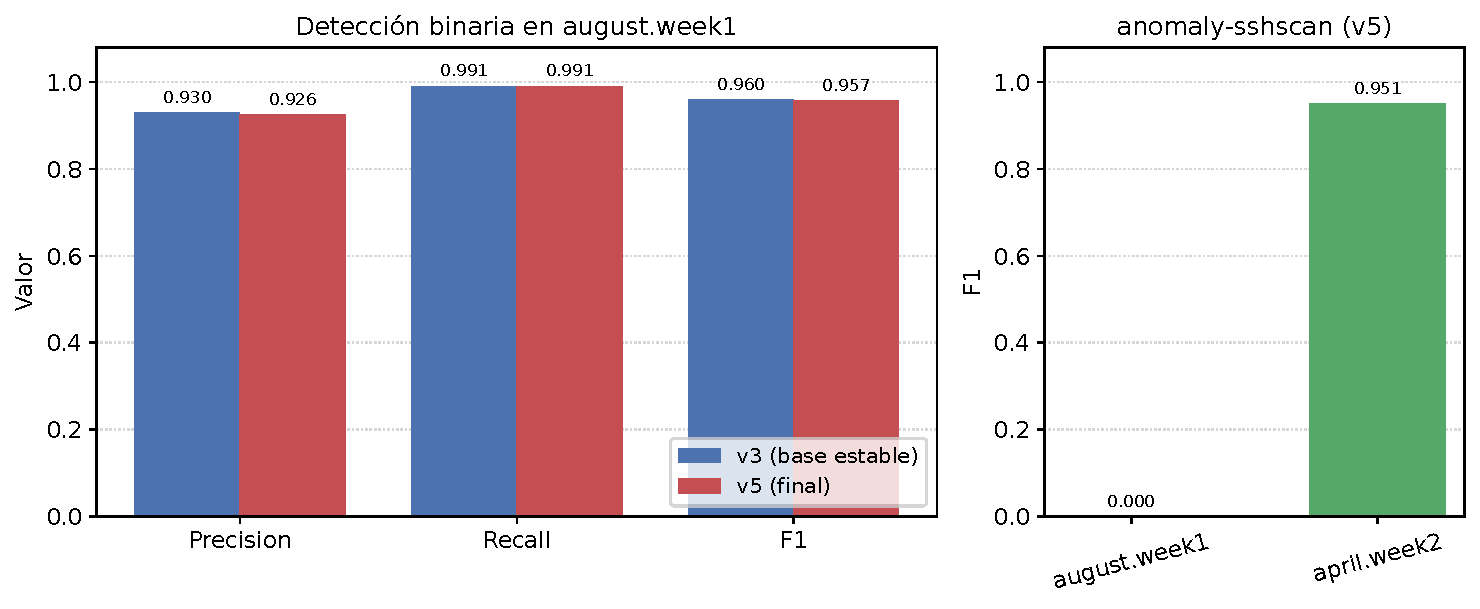
\includegraphics[width=\textwidth]{imagenes/fig_v3_vs_v5_binaria.pdf}
\caption{Comparacion del rendimiento binario de las versiones v3 y v5 y efecto del contexto global en la deteccion de \texttt{anomaly-sshscan}. Fuente: elaboración propia.}
\label{fig:v3_vs_v5}
\end{figure}

La Figura~\ref{fig:v3_vs_v5} resume esta comparación binaria entre la v3 y la v5 y el salto en la detección del escaneo SSH al pasar del contexto local al global. La v5 no es un detector perfecto. Su valor está en que mantiene el rendimiento de la v3 en el núcleo de ataques y, además, recupera una familia que la v3 no detectaba en absoluto, a costa de algún falso positivo en las semanas sin ese ataque. La v4, en cambio, exploró un reparto de confianza en la familia de botnet que no mejoró de forma concluyente, por lo que no se adopta.

\section{Resultados por familia de ataque}
\label{sec:exp_familia}

La Tabla~\ref{tab:exp_familia} recoge los resultados por familia en \texttt{august.week1}, el conjunto principal de estudio. Las cifras de precisión, recall y $F_1$ se derivan de los recuentos del resumen (predichas, etiquetadas y aciertos) de cada subtipo.

\begin{table}[ht]
\centering
\small
\begin{tabular}{|l|r|r|r|c|c|c|}
\hline
\textbf{Familia} & \textbf{Predichas} & \textbf{Etiquetadas} & \textbf{Aciertos} & \textbf{P} & \textbf{R} & \textbf{F1} \\
\hline
anomaly-udpscan & 1\,067\,045 & 1\,001\,413 & 1\,001\,219 & 0,938 & 1,000 & 0,968 \\
\hline
scan11 & 133\,989 & 102\,572 & 102\,220 & 0,763 & 0,997 & 0,864 \\
\hline
scan44 & 399\,411 & 382\,351 & 304\,396 & 0,762 & 0,796 & 0,779 \\
\hline
dos & 217\,724 & 247\,230 & 120\,635 & 0,554 & 0,488 & 0,519 \\
\hline
nerisbotnet & 16\,462 & 99\,762 & 4\,420 & 0,269 & 0,044 & 0,076 \\
\hline
anomaly-sshscan & 8\,397 & 44 & 0 & 0,000 & 0,000 & 0,000 \\
\hline
\end{tabular}
\caption{Resultados por familia en \texttt{august.week1}, derivados del resumen por familia de la v5 (trazas predichas, etiquetadas y aciertos de cada clase). El escaneo SSH se evalúa realmente en \texttt{april.week2} (Tabla~\ref{tab:exp_sshscan}).}
\label{tab:exp_familia}
\end{table}
% [REVISAR: en el resumen, los aciertos a nivel de familia vertical_scan (410782) no coinciden exactamente con la suma de aciertos de scan11+scan44 (102220+304396=406616), diferencia de 4166, por distinto criterio de acierto entre nivel familia y subtipo. No afecta a las cifras por subtipo mostradas.]

\begin{figure}[ht]
\centering
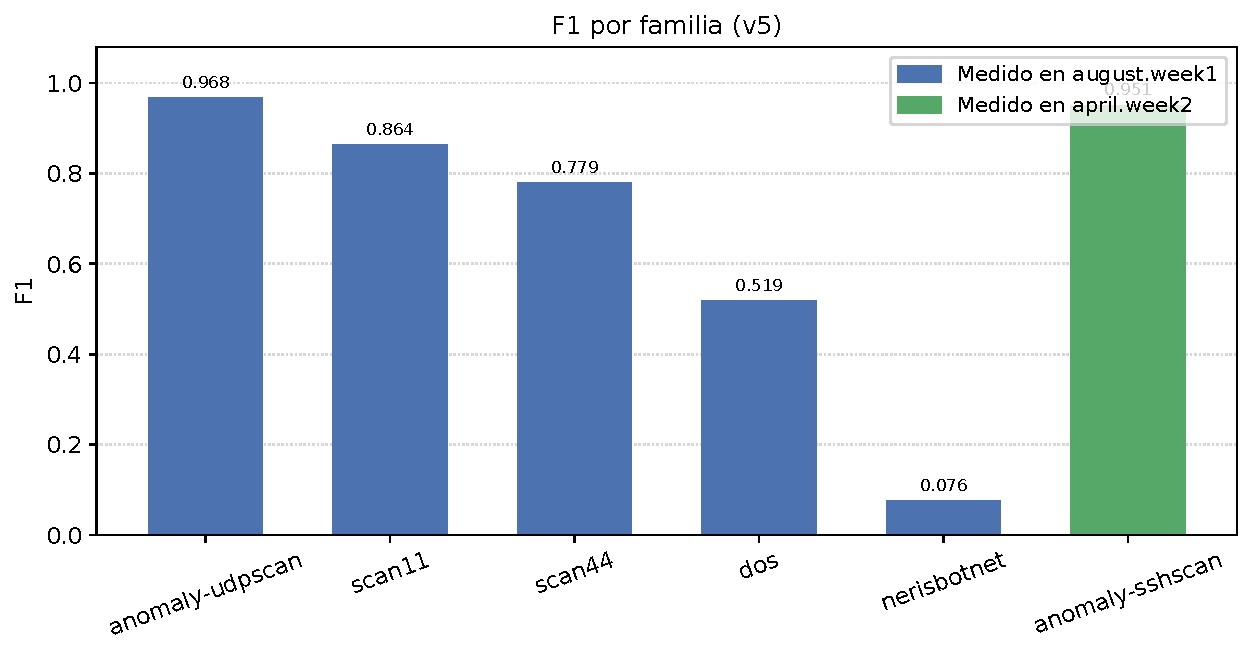
\includegraphics[width=0.9\textwidth]{imagenes/fig_f1_por_familia.pdf}
\caption{F1 por familia de ataque para la version v5 del clasificador. Fuente: elaboración propia.}
\label{fig:f1_familia}
\end{figure}

La Figura~\ref{fig:f1_familia} muestra de un vistazo el $F_1$ de cada familia con la v5. El comportamiento por familia es el siguiente:

\begin{itemize}
  \item \textbf{anomaly-udpscan}: es la familia mejor detectada en estos datos (F1 0,968, recall 1,000). El patrón es muy claro en \texttt{august.week1}. Sin embargo, no aparece en las otras semanas disponibles, por lo que su generalización fuera del conjunto principal de estudio no se ha podido comprobar y queda como trabajo futuro.
  \item \textbf{scan11} y \textbf{scan44}: los escaneos verticales se detectan bien a nivel agregado (F1 0,864 y 0,779). El punto débil está en la frontera entre ambos subtipos, ya que parte de \texttt{scan44} se confunde, lo que explica su recall más bajo (0,796).
  \item \textbf{dos}: presenta un rendimiento intermedio (F1 0,519). La concentración de tráfico es detectable solo en parte, y se solapa con otros comportamientos intensivos de red, lo que reduce tanto la precisión como el recall.
  \item \textbf{nerisbotnet}: es la familia más difícil del núcleo (F1 0,076, recall 0,044). La coordinación entre nodos no siempre es visible usando únicamente metadatos de flujo, y el sistema recupera muy pocas instancias.
  \item \textbf{anomaly-sshscan}: en \texttt{august.week1} no es evaluable de forma representativa, ya que apenas hay 44 trazas etiquetadas y no se obtiene ningún acierto. Su evaluación real se hace en \texttt{april.week2}.
\end{itemize}

La recuperación del escaneo SSH es el cambio más visible de la v5. La Tabla~\ref{tab:exp_sshscan} muestra su rendimiento en \texttt{april.week2}, la semana donde esta familia aparece con muchas más muestras.

\begin{table}[ht]
\centering
\small
\begin{tabular}{|l|r|r|r|c|c|c|}
\hline
\textbf{Familia (semana)} & \textbf{Predichas} & \textbf{Etiquetadas} & \textbf{Aciertos} & \textbf{P} & \textbf{R} & \textbf{F1} \\
\hline
anomaly-sshscan (\texttt{april.week2}) & 26\,599 & 29\,298 & 26\,580 & 0,999 & 0,907 & 0,951 \\
\hline
\end{tabular}
\caption{Escaneo SSH detectado por la v5 en \texttt{april.week2}, obtenido del resumen de generalización de esa semana.}
\label{tab:exp_sshscan}
\end{table}

El escaneo SSH, que no se detectaba con el contexto local disponible en \texttt{august.week1}, pasa a detectarse con un F1 de 0,951 cuando se observa el comportamiento global de cada origen. Es donde mejor se ve lo que aporta mirar el contexto y no solo el flujo aislado.

Por último, la clase de campaña SMTP de baja evidencia se descartó del análisis principal, como se explicó en los Capítulos~\ref{cap:herramientas_datos} y~\ref{cap:algoritmos}. No forma parte de los resultados activos. En los resúmenes su número de aciertos es nulo, coherente con el límite de NetFlow para este tipo de comportamiento, ya que no recoge el contenido de los mensajes. Por eso no se considera un resultado del trabajo.

\section{Comparación con Machine Learning clásico}
\label{sec:exp_ml}

Como referencia secundaria, se entrenaron varios modelos clásicos de aprendizaje automático sobre una muestra equilibrada por clases: regresión logística, $k$ vecinos más cercanos (KNN), máquinas de vectores soporte (SVM) y un perceptrón multicapa (MLP). Estos modelos se utilizan como \textbf{línea base de comparación}, no como sustituto del clasificador contextual \cite{buczak2016survey}. La Tabla~\ref{tab:exp_ml} resume su rendimiento.

\begin{table}[ht]
\centering
\small
\begin{tabular}{|l|c|c|}
\hline
\textbf{Modelo} & \textbf{F1 macro (8 clases originales)} & \textbf{F1 macro (clases activas)} \\
\hline
KNN & 0,877 & 0,942 \\
\hline
MLP & 0,803 & 0,889 \\
\hline
SVM & 0,660 & 0,780 \\
\hline
Regresión logística & 0,615 & 0,760 \\
\hline
\end{tabular}
\caption{Línea base de ML clásico: F1 macro sobre las 8 clases originales (incluían \texttt{anomaly-spam} y \texttt{blacklist}) frente al cálculo sobre las clases activas. Se obtiene del resumen por clase del baseline, antes y después de excluir las clases no activas. El F1 macro es la media del F1 por clase.}
\label{tab:exp_ml}
\end{table}

El baseline principal se calcula sobre las \textbf{clases activas} del trabajo: el tráfico de fondo (\emph{background}) y los cinco tipos de ataque presentes en la muestra (\texttt{anomaly-udpscan}, \texttt{dos}, \texttt{nerisbotnet}, \texttt{scan11} y \texttt{scan44}). Se dejan fuera dos etiquetas que no forman parte del objetivo principal. La primera es \texttt{anomaly-spam}, descartada metodológicamente (Capítulos~\ref{cap:herramientas_datos} y~\ref{cap:algoritmos}). La segunda es \texttt{blacklist}, que está en el dataset pero no es una familia de ataque activa del TFG, así que queda fuera de la tabla principal de comparación. El escaneo SSH (\texttt{anomaly-sshscan}) no entra en este baseline por su escasez de muestras en el conjunto principal de estudio, coherente con su evaluación específica en \texttt{april.week2}.

Como el F1 macro es la media del F1 por clase, recalcularlo sobre las clases activas no altera las métricas por clase: simplemente deja de promediar las clases excluidas. El recálculo parte del resumen por clase ya calculado, vuelve a promediar el F1 únicamente sobre las clases activas y guarda el resultado aparte, sin reentrenar ningún modelo ni sobrescribir los resultados originales. Partir de ese resumen aísla el efecto exacto de excluir esas clases, manteniendo el mismo muestreo, los mismos modelos y las mismas predicciones. La Tabla~\ref{tab:exp_ml} muestra el efecto: al dejar fuera dos clases en las que varios modelos rendían mal (en especial la regresión logística y la SVM), el F1 macro sube en todos los modelos. Por ejemplo, la regresión logística pasa de 0,615 a 0,760.

En cualquier caso, el rendimiento del baseline hay que leerlo con cuidado \cite{sommer2010outside}. Son modelos \textbf{supervisados}, que necesitan etiquetas para entrenar, y se evalúan sobre una muestra equilibrada, más favorable que el tráfico real desbalanceado. Además, ofrecen menos trazabilidad que el clasificador contextual: predicen bien, pero no explican cada decisión con una señal observable del tráfico. La diferencia que importa no es la métrica, sino el equilibrio entre \textbf{rendimiento predictivo} y \textbf{explicabilidad}. Este trabajo prioriza lo segundo e incluye el aprendizaje automático clásico como una referencia honesta, no como el enfoque principal.

\section{Pruebas de generalización}
\label{sec:exp_generalizacion}

En este trabajo, generalizar significa comprobar si el clasificador funciona sobre semanas que no se usaron para formular las reglas, sin reajustarlas después. El alcance es limitado: se trata de una generalización \textbf{parcial dentro de UGR'16}, no de una validación en cualquier red real. La Tabla~\ref{tab:exp_general} resume la detección binaria de la v5 en los tres conjuntos.

\begin{table}[ht]
\centering
\small
\begin{tabular}{|l|c|c|c|p{4.6cm}|}
\hline
\textbf{Semana} & \textbf{P} & \textbf{R} & \textbf{F1} & \textbf{Familias presentes} \\
\hline
\texttt{august.week1} & 0,926 & 0,991 & 0,957 & Núcleo (udpscan, scan11/scan44, dos, nerisbotnet). \\
\hline
\texttt{august.week2} & 0,872 & 0,747 & 0,805 & Escaneo vertical, dos, nerisbotnet. Sin udpscan. \\
\hline
\texttt{april.week2} & 0,845 & 0,903 & 0,873 & Sobre todo escaneo SSH. \\
\hline
\end{tabular}
\caption{Detección binaria de la v5 por semana, obtenida de los resúmenes binarios de la v5 en cada semana evaluada.}
\label{tab:exp_general}
\end{table}

\begin{figure}[ht]
\centering
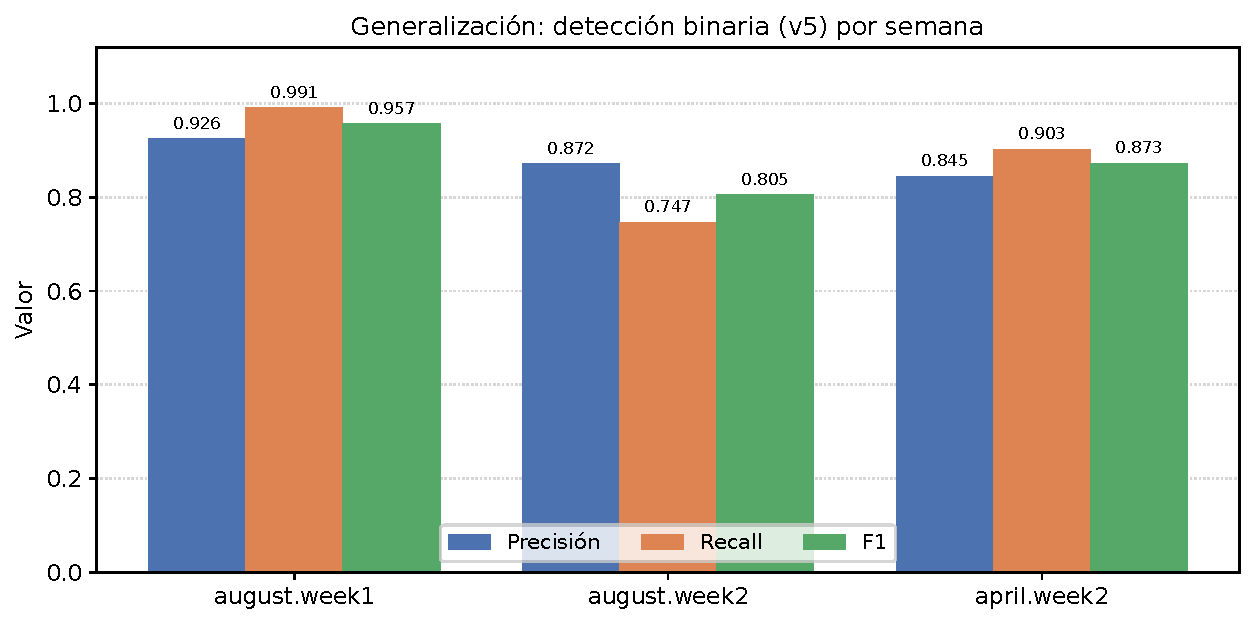
\includegraphics[width=0.9\textwidth]{imagenes/fig_generalizacion_semanas.pdf}
\caption{Resultados binarios de generalizacion por semana evaluada. Fuente: elaboración propia.}
\label{fig:generalizacion}
\end{figure}

La Figura~\ref{fig:generalizacion} compara la precisión, el recall y el $F_1$ binarios de la v5 en las tres semanas. En \texttt{august.week2} se observa que el núcleo de escaneos generaliza de forma razonable: el escaneo vertical mantiene un buen recuento de aciertos (62\,961 sobre 73\,830 trazas etiquetadas como escaneo vertical). El recall binario baja a 0,747, en parte porque esta semana contiene una gran cantidad de tráfico de campaña SMTP que el sistema no resuelve y que penaliza el recall agregado. Recordemos que el escaneo UDP \textbf{no aparece} en esta semana, por lo que su generalización no puede comprobarse.

En \texttt{april.week2}, que contiene principalmente escaneo SSH, la v5 alcanza una detección binaria de F1 0,873, y la familia de escaneo SSH se detecta con F1 0,951 (Tabla~\ref{tab:exp_sshscan}). En esta semana, el tercer pase de la v5 funciona como se esperaba: de las 26\,580 detecciones por fan-out, ninguna se contabiliza como falso positivo del propio pase. Esto indica, dentro de estos datos, que la mejora de la v5 no depende únicamente del conjunto principal de estudio.

No se afirma una generalización universal. Solo se observa que el núcleo de escaneos se mantiene en otra semana y que la mejora del escaneo SSH se confirma en una semana independiente, dentro de los límites del propio dataset.

\section{Discusión de resultados}
\label{sec:exp_discusion}

En conjunto, las familias mejor detectadas son las que presentan un \textbf{patrón estructural claro} en los metadatos: el escaneo UDP y los escaneos verticales. Las más difíciles son las que dependen de información que NetFlow no captura bien, como la coordinación de una red de bots o comportamientos que solo se ven al observar periodos más largos.

El \textbf{contexto temporal y global} es la idea que más se repite en estos resultados. El escaneo SSH lo resume bien: con una mirada local apenas era visible, mientras que con la agregación por origen se detecta con mucha más claridad. La \textbf{explicabilidad} también cuenta, porque cada decisión se asocia a una señal que puede revisarse. Esto permite entender tanto los aciertos como los errores, por ejemplo, por qué la v5 genera falsos positivos de SSH en semanas sin ese ataque etiquetado.

Los \textbf{límites de NetFlow} aparecen de forma recurrente: sin contenido, hay familias que no se separan bien del tráfico normal. Además, la evaluación depende de las etiquetas disponibles. Si parte del tráfico de fondo contiene comportamientos anómalos no etiquetados, el sistema los contará como falsos positivos aunque su estructura pueda parecer sospechosa. Por eso los errores no deben leerse únicamente como fallos del clasificador, sino también como una consecuencia de trabajar con trazas reales y etiquetas cerradas.

La diferencia con el aprendizaje automático supervisado también se ve aquí. Un modelo supervisado puede puntuar más alto en una muestra equilibrada, pero no ofrece la misma trazabilidad que un conjunto de reglas explícitas. En este TFG, la interpretabilidad es una parte central de la propuesta, no un añadido secundario.

\section{Amenazas a la validez}
\label{sec:exp_amenazas}

Los resultados de este capítulo deben leerse teniendo en cuenta varias amenazas a su validez, que conviene declarar de forma abierta:

\begin{itemize}
  \item \textbf{Dependencia de UGR'16.} Toda la evaluación se apoya en un único dataset. Aunque es tráfico real de un proveedor de servicios de Internet, los resultados no tienen por qué trasladarse tal cual a otras redes, con distinta composición de tráfico y otros ataques.
  \item \textbf{Desbalance extremo.} El tráfico normal domina con mucho sobre el malicioso. Esto obliga a interpretar las métricas con cuidado y es la razón por la que se descarta la exactitud como medida principal, en favor de la precisión, el recall y el $F_1$.
  \item \textbf{Dependencia de las etiquetas.} La salida del sistema se compara siempre con las etiquetas del dataset. Si un flujo marcado como \emph{background} tiene en realidad una estructura anómala, se cuenta como falso positivo aunque su comportamiento se parezca al de un ataque. Parte de las falsas alarmas puede explicarse así.
  \item \textbf{Ausencia de contenido.} Al trabajar con NetFlow no hay payload. Esto limita de forma estructural la detección de las familias cuya naturaleza solo se aprecia mirando el contenido, y no los metadatos.
  \item \textbf{Familias con pocas muestras.} El escaneo SSH apenas tiene trazas etiquetadas en \texttt{august.week1} (44) y \texttt{august.week2} (5), por lo que su evaluación representativa se concentra en \texttt{april.week2}. Con tan pocos ejemplos en una semana no se pueden extraer conclusiones sólidas sobre ella.
  \item \textbf{Sesgo de diseño.} Las reglas se formularon observando ventanas del propio dataset, lo que puede favorecer los resultados sobre esos mismos datos. Es parte del motivo por el que se reservan otras semanas para la generalización.
  \item \textbf{Generalización limitada.} Solo se ha probado en otras semanas de UGR'16, nunca en una red distinta. Además, el escaneo UDP no aparece fuera del conjunto principal de estudio, de modo que su generalización queda sin comprobar.
  \item \textbf{No equivale a producción.} La evaluación se hace sobre ventanas y capturas ya disponibles, no sobre un flujo continuo en tiempo real, que plantearía retos añadidos de rendimiento y de decisión en caliente.
\end{itemize}

\section{Conclusiones del capítulo}
\label{sec:exp_conclusion}

Los experimentos muestran que el clasificador contextual separa bien ataque y tráfico normal en el conjunto principal de estudio (F1 binario 0,957 con la v5) y que detecta con solvencia las familias con patrones más claros, especialmente el escaneo UDP (F1 0,968) y los escaneos verticales. La versión \textbf{v5 integrated} queda como versión final: mantiene un rendimiento cercano al de la base estable v3 y recupera el escaneo SSH (F1 0,951 en \texttt{april.week2}), que antes no se detectaba de forma efectiva. Esta mejora tiene un coste en falsos positivos en semanas sin escaneo SSH etiquetado, por lo que no se presenta como una mejora absoluta en todas las métricas. La v4 se mantiene solo como experimento intermedio.

También se reconocen los límites del enfoque. La red de bots es difícil de detectar usando solo metadatos, y el escaneo UDP no ha podido evaluarse fuera del conjunto principal de estudio. Además, algunas alertas contabilizadas como falsos positivos podrían corresponder a comportamientos anómalos no etiquetados como ataque, aunque en la evaluación se respeten siempre las etiquetas originales del dataset.

El baseline de aprendizaje automático clásico se ha recalculado sobre las clases activas, dejando fuera la clase descartada y la etiqueta de listas negras, de modo que la comparación es más coherente con la metodología del trabajo. Frente a los modelos supervisados, que pueden puntuar alto pero ofrecen menos trazabilidad, la propuesta prioriza la explicabilidad. Esa idea de explicar cada decisión es la que recoge la aplicación web interactiva del Capítulo~\ref{cap:web}.
